\documentclass[11pt]{article}

% arXiv preprint: non-anonymous, with page numbers.
\usepackage[preprint]{acl}

\usepackage{times}
\usepackage{latexsym}
\usepackage[T1]{fontenc}
\usepackage[utf8]{inputenc}
\usepackage{amsmath}
\usepackage{microtype}
\usepackage{inconsolata}
\usepackage{graphicx}
\usepackage{booktabs}
\usepackage{multirow}

% The released figure PDFs are the ones the website serves, and they are
% tracked; results/figures/ is regenerated output and is not.
\graphicspath{{../site/public/figures/}}

% Both figures are wide floats. At LaTeX's defaults they do not clear
% \floatpagefraction and are deferred past the bibliography. Letting a float
% page be mostly float keeps them in the body, beside the text that refers to
% them.
\renewcommand{\topfraction}{0.92}
\renewcommand{\textfraction}{0.07}
\renewcommand{\floatpagefraction}{0.72}
\setcounter{topnumber}{2}
\setcounter{totalnumber}{3}
\setlength{\textfloatsep}{10pt plus 2pt minus 2pt}
\setlength{\intextsep}{10pt plus 2pt minus 2pt}
\setlength{\abovecaptionskip}{4pt}

\newcommand{\us}{\ensuremath{\mu}s}
\newcommand{\code}[1]{\texttt{\small #1}}

\title{Attention Kernel Portability Across Six GPUs and Two Inference Regimes:\\
       A Measurement Study}

\author{Srivatsan Sarvesan \\
  University of California, San Diego \\
  \texttt{ssarvesan@ucsd.edu} \\}

\begin{document}
\maketitle

\begin{abstract}
We study whether an attention backend selected on one GPU remains a good choice
on another. We benchmark forward prefill and single-token KV-cache decode on six
NVIDIA GPUs with fixed library versions. A backend is the separated winner of a
configuration when the runner-up is at least 10\% slower and the lower bound of
a 95\% bootstrap interval on the latency ratio exceeds 1. This holds in 128 of
447 forward-prefill and 409 of 1{,}203 decode configurations. Among separated
comparisons across Ampere, Ada and Hopper GPUs, the winner changes in 27 of 64
prefill comparisons and 29 of 289 decode comparisons. Reusing the source GPU's
choice on the target costs a median 1.002$\times$ for prefill and 1.000$\times$
for decode, with 95th percentiles of 1.610$\times$ and 1.325$\times$. In some
cases the source's choice cannot run on the target at all, and we report those
separately. Each GPU was measured on its own host, so the results do not
separate architecture from host effects.
\end{abstract}

\section{Introduction}

A practitioner choosing an attention kernel usually reads a benchmark run on a
single GPU. Does the winner of that benchmark stay the winner on a different
GPU?

Serving systems usually assume it does. They fix an attention backend by a
preference order and use that order on every device they deploy to. If the
ranking is a property of the kernel, that is fine. If it is a property of the
kernel and device together, an order tuned on one GPU may be wrong on another.

We time 10 prefill and 6 decode implementations over 403 configurations on the
six GPUs in Table~\ref{tab:devices}. The 73{,}230 attempts give 11{,}835 usable
(GPU, configuration, implementation) medians.\footnote{Code:
\url{https://github.com/Srivatsan6923/attention-kernel-portability}. The
measurements are in release
\url{https://github.com/Srivatsan6923/attention-kernel-portability/releases/tag/v1.2}
with SHA-256 checksums.}
Every claim compares a ranking within one device against the ranking within
another. We never claim that one device is faster than another.

The study makes two contributions. The first is a measurement protocol that
records which kernel actually ran and names a winner only when it is separated
from the runner-up. The second is the finding that a backend choice holds only
for the GPU, regime and library versions it was measured on.

\section{Background and related work}

FlashAttention \citep{dao2022flashattention} keeps the $N \times N$ score matrix
out of HBM and is evaluated on A100. FlashAttention-2
\citep{dao2023flashattention2} is also evaluated on A100, and FlashAttention-3
\citep{shah2024flashattention3} targets H100 only. Each reports results on the
GPU its authors measured, which is the practice this study tests.
Flash-Decoding \citep{dao2023flashdecoding} adds split-KV for single-token
queries on A100, and FlashInfer \citep{ye2025flashinfer} builds it into a
serving engine evaluated on A100 and H100.

Compiler and kernel benchmarks follow the same pattern. The PyTorch 2 paper
\citep{ansel2024pytorch2} evaluates TorchInductor, which generates Triton
\citep{tillet2019triton}, on one A100. KernelBench \citep{ouyang2025kernelbench}
profiles 250 PyTorch workloads on an L40S, and TritonBench
\citep{li2025tritonbench} evaluates 184 Triton operators on an A100. Serving
systems such as vLLM \citep{kwon2023vllm}, Sarathi-Serve
\citep{agrawal2024sarathi} and DistServe \citep{zhong2024distserve} are
evaluated on A100, and Splitwise \citep{patel2024splitwise} on A100 and H100.
TVM \citep{chen2018tvm} and Ansor \citep{zheng2020ansor} instead search for an
implementation per target, which treats the best implementation as a property
of the hardware. In HPC the question is well studied.
\citet{williams2009roofline} give per-architecture performance ceilings, and
\citet{pennycook2016metric} and \citet{deakin2019portability} define
performance portability over a stated set of platforms.

\section{Study design}

\paragraph{Implementations and grid.} The prefill set is a naive PyTorch
reference, a \code{torch.compile} path in three variants, the three PyTorch SDPA
backends (memory-efficient, flash and cuDNN), the Triton fused-attention
tutorial kernel with a small BF16 change, and FlashAttention 2 and 3. The decode
set is a naive KV-cache implementation, an Inductor path, SDPA,
\code{flash\_attn\_with\_kvcache}, FlashInfer, and FlashAttention prefill at
query length 1. A \emph{cell} is one configuration, defined by regime, batch,
query and KV head counts, head dimension, sequence length, dtype, forward or
forward-plus-backward, launch mode, cache state and causality. The full grid
has 159 prefill and 244 decode cells. Table~\ref{tab:devices} gives per-device
coverage.

\paragraph{Timing protocol.} Backend order is randomised per configuration, and
each backend's timing blocks run back to back. Because backends are not
interleaved, we do not assume host or thermal effects cancel within a
comparison. In eager mode, each block's CUDA-event time is divided by its call
count. We take the median over blocks within a process launch, then the median
over launches. Blocks target about 200~\us{}. For cold-cache cells, L2 is
flushed once before each block, so only the first call in a block is fully
cold. CUDA-graph cells are timed with Triton's \code{do\_bench\_cudagraph}.
Confidence intervals come from a 2000-draw bootstrap that resamples whole
process launches, because calls within a launch share clock and thermal state.
The median between-process coefficient of variation (CV) is 0.011 on A10
(n=1871) and 0.026 on H100 (n=2474).

Processes are pinned to the NUMA node closest to the GPU. In two runs of the
H100 decode grid that differ only in pinning, the median between-process CV
over 966 matched (cell, implementation) pairs falls from 0.112 unpinned to
0.034 pinned, and the share above 25\% CV falls from 30.7\% to 9.9\%. These
numbers use block-level timing and are not directly comparable with the
per-call CVs above.

\paragraph{Definitions.} Let $t_{g,c,b,r}$ be the median latency of an attention
call in process launch $r$, for GPU $g$, configuration $c$ and backend $b$. The
reported latency is the median over launches,
%
\begin{equation}
T_{g,c,b} \;=\; \operatorname*{median}_{r}\; t_{g,c,b,r} .
\label{eq:lat}
\end{equation}
%
With $b_1$ and $b_2$ the fastest and second-fastest eligible backends at
$(g,c)$, the separation ratio and rule are
%
\begin{equation}
R_{g,c} \;=\; \frac{T_{g,c,b_2}}{T_{g,c,b_1}} ,
\label{eq:ratio}
\end{equation}
\vspace{-1.1em}
\begin{equation}
\mathrm{Sep}(g,c) \;=\; \mathbf{1}\!\left[\,R_{g,c} \ge 1.10 \;\wedge\;
L_{95}(R_{g,c}) > 1 \,\right],
\label{eq:sep}
\end{equation}
%
where $L_{95}$ is the lower end of a 95\% bootstrap interval on the same ratio.
Both conditions are required. Failing the rule does not show that the backends
are equal. It means no fastest backend could be established. In all 2{,}082
cells used here, the fastest and second-fastest backends ran in the same set of
launches. In the wider scan over every implementation pair, 50 of 29{,}304
pairs, all on the RTX 5090 and all involving the naive reference, lost a launch
to an out-of-memory failure. Those pairs are compared on the launches both
backends share.

Let $\mathcal{B}_{g,c}$ be the backends with a usable measurement at $(g,c)$ and
$b^{*}_{g,c}$ the winner. Let $\mathcal{E}$ be the set of matched comparisons
$(g,h,c)$ where $c$ was measured on both GPUs and
$\mathrm{Sep}(g,c) = \mathrm{Sep}(h,c) = 1$. The winner-change rate is
%
\begin{equation}
\mathrm{WCR} \;=\;
\frac{\sum_{(g,h,c)\in\mathcal{E}} \mathbf{1}\!\left[b^{*}_{g,c} \neq b^{*}_{h,c}\right]}
     {\lvert \mathcal{E} \rvert} .
\label{eq:wcr}
\end{equation}
%
The common-backend variant limits each comparison to
$\mathcal{B}_{g,c} \cap \mathcal{B}_{h,c}$ for that configuration and
recomputes $b^{*}$ and $\mathrm{Sep}$ inside that set.

The cost of reusing GPU $g$'s choice on GPU $h$ is
%
\begin{equation}
C_{g \rightarrow h,\,c} \;=\;
\frac{T_{h,c,\,b^{*}_{g,c}}}{\min_{b \in \mathcal{B}_{h,c}} T_{h,c,b}} .
\label{eq:transfer}
\end{equation}
%
A value of 1.20 means the source's choice is 20\% slower than the fastest
backend on the target. When $b^{*}_{g,c} \notin \mathcal{B}_{h,c}$ the ratio is
undefined. We count those cases and never substitute the target's own best.

\paragraph{Correctness gate.} Every implementation is checked against a
reference, and only rows that pass enter a ranking. Of 73{,}230 attempts,
54{,}213 (74.0\%) completed with status \code{OK}. Of those, 54{,}098 passed
the check and are eligible. The other 115 belong to one class that was never
checked on its own device and are excluded. Of the remaining attempts, 16{,}326
were \code{UNSUPPORTED}, 1{,}590 were skipped by an out-of-memory predictor,
950 raised a run-time error (all FlashInfer on the RTX 5090,
Section~\ref{sec:mech}), and 151 ran out of memory despite passing the
predictor. No correctness check failed. Bandwidth is measured on each host with
a copy benchmark, not taken from a datasheet.

\begin{table}[tb]
\centering
\small
\setlength{\tabcolsep}{3.2pt}
\begin{tabular}{lllrrr}
\toprule
GPU & cc & family & BW & \shortstack{planned\\repeats} & cells \\
 & & & (GB/s) & pre/dec & pre/dec \\
\midrule
A100     & 8.0  & Ampere    & 1732.8 & 5/5 & 144/192 \\
A10      & 8.6  & Ampere    &  483.3 & 5/5 & 144/191 \\
L40      & 8.9  & Ada       &  644.4 & 3/3 & 144/192 \\
L40S     & 8.9  & Ada       &  644.4 & 5/5 & 144/192 \\
H100     & 9.0  & Hopper    & 2979.7 & 5/5 & 159/244 \\
RTX 5090 & 12.0 & Blackwell & 1517.5 & 5/5 & 144/192 \\
\bottomrule
\end{tabular}
\caption{GPUs and coverage. Bandwidth comes from a copy benchmark on each host.
\emph{Planned repeats} are separate process launches per configuration, for
prefill and decode. L40 kept a median of two usable repeats. \emph{Cells} counts
configurations with at least one eligible measurement.}
\label{tab:devices}
\end{table}

\section{Dispatch validation}

A latency says something about a kernel only if that kernel actually ran. We
tried to record the launched kernel names for every timed row and got a
readable trace for 36{,}054 of the 54{,}213 \code{OK} attempts (66.5\%).
Grouping rows by the fields that decide dispatch (implementation, GPU, head
dimension, dtype, GQA ratio, mode and launch) gives 651 dispatch classes, and
625 of them (96.0\%) have at least one traced row. A class confirms the kernel
family only. Within a class the exact kernel can change with batch, for example
between \code{flash\_fwd\_splitkv\_combine} and \code{flash\_fwd}, but the
family is always the one requested.

Among traced rows, the requested kernel family is missing from the trace in 162
cases, a mismatch rate of 0.449\%. Over all \code{OK} rows that is 0.299\%. We
treat the untraced 33.5\% as unknown, not as matching. The mismatches cluster,
with 66 of the 162 coming from the SDPA memory-efficient backend on H100.

For TorchInductor, 3{,}645 of 17{,}537 Inductor rows recorded the
\code{fuse\_attention} counter, and it was 0 on every one of them across all six
GPUs. Inductor's attention-fusion pattern therefore never fired on those rows.
The counter does not tell the whole story, though. 45 traced Inductor rows on
H100, from 6 distinct cells, did launch a flash kernel.

\section{Portability}
\label{sec:port}

\begin{figure*}[tb]
\centering
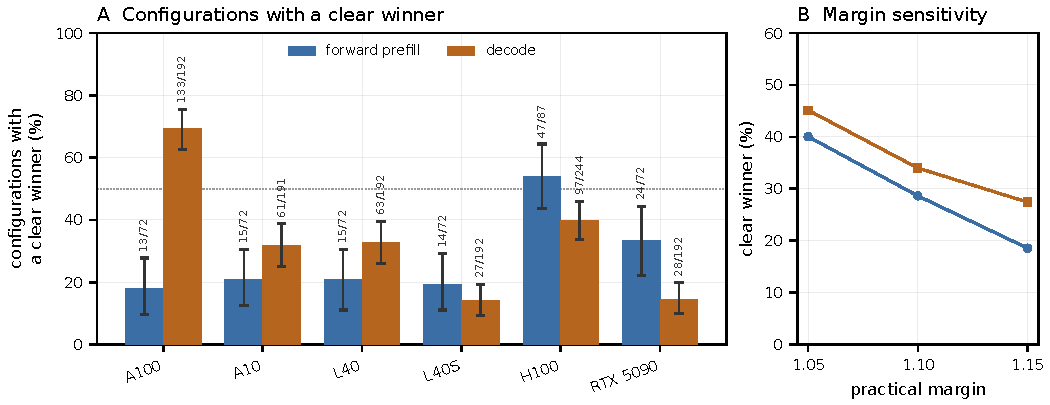
\includegraphics[width=\textwidth]{figA_separation.pdf}
\caption{Share of configurations with a clear (separated) winner, by GPU.
Whiskers are 95\% intervals, and the counts above each bar are separated over
total configurations. Workload counts differ by GPU. Panel B shows the pooled
rate at margins of 1.05, 1.10 and 1.15.}
\label{fig:sep}
\end{figure*}

\begin{figure*}[tb]
\centering
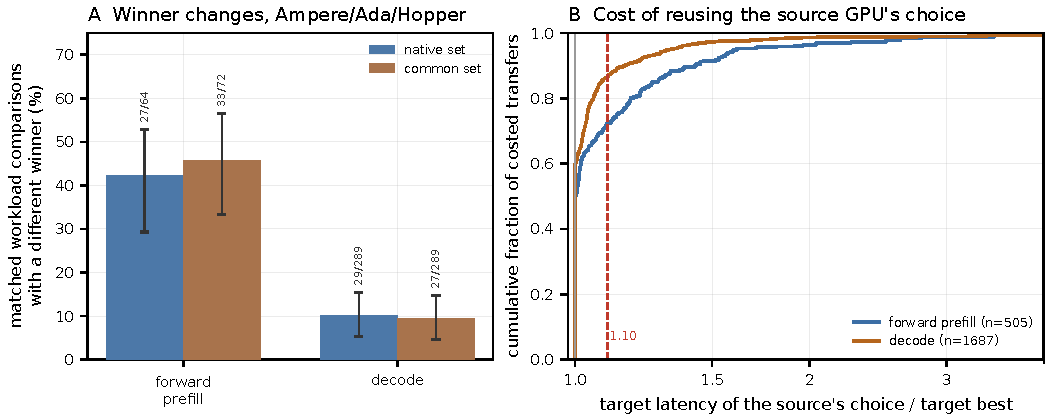
\includegraphics[width=\textwidth]{figB_transfer.pdf}
\caption{Left, the winner-change rate over the ten Ampere, Ada and Hopper GPU
pairs, using each GPU's own backends (native set) and only the backends both
GPUs ran (common set). Right, the distribution of reuse cost over all ordered
pairs of the six GPUs where the source has a separated winner. In 85 of 590
prefill and 287 of 1{,}974 decode cases the source's choice had no usable
timing on the target, and these are not plotted. The cost distribution
includes cases where the winner did not change.}
\label{fig:transfer}
\end{figure*}

\paragraph{Most configurations have no clear winner.} Only 28.6\% of
forward-prefill and 34.0\% of decode configurations have a separated winner
(128 of 447 and 409 of 1{,}203). Figure~\ref{fig:sep} gives the rate per GPU.
A flip between two backends within a few percent of each other is not a
measured difference, so Table~\ref{tab:flips} reports every rate over all
shared configurations and over those separated on both GPUs.

\paragraph{Prefill winners change far more often than decode winners.}
Table~\ref{tab:flips} pools the ten pairs among A10, A100, L40, L40S and H100.
Over all shared configurations the two regimes look similar (66.0\% and 52.1\%).
Keeping only separated comparisons pulls them apart. Prefill changes winner in
27 of 64 comparisons (42.2\%) and decode in 29 of 289 (10.0\%). Restricting each
pair to the backends both GPUs ran, and recomputing winners in that set, gives
33 of 72 for prefill and 27 of 289 for decode. This restriction removes
backends that only one GPU could run, such as FlashAttention 3, and it does not
lower the prefill rate. Figure~\ref{fig:transfer} shows what reusing a choice costs.
The median reused choice is 1.002$\times$ the target's best in prefill and
1.000$\times$ in decode, but the 95th percentiles are 1.61$\times$ and
1.32$\times$.

\paragraph{The RTX 5090.} The lower half of Table~\ref{tab:flips} repeats the
calculation for the five pairs that include the RTX 5090. Decode changes winner
in 63 of 85 comparisons and prefill in 16 of 30. In most of the decode cases
the other GPU's winner is FlashInfer, which produced no timing on the 5090
(Section~\ref{sec:mech}). We did not measure what FlashInfer would have cost
there, so we do not attribute the high rate to architecture.

\begin{table}[tb]
\centering
\small
\setlength{\tabcolsep}{1.5pt}
\begin{tabular}{llrrrr}
\toprule
 & & \multicolumn{2}{c}{all shared cells} & \multicolumn{2}{c}{separated both} \\
\cmidrule(lr){3-4}\cmidrule(lr){5-6}
device set & regime & n & flip & n & flip [95\% CI] \\
\midrule
\multirow{2}{*}{Amp/Ada/Hop} & prefill & 720 & 66.0\% & 64 & 42.2\% [29, 53] \\
                             & decode  & 1916 & 52.1\% & 289 & 10.0\% [5, 15] \\
\midrule
\multirow{2}{*}{5090 vs rest} & prefill & 360 & 65.8\% & 30 & 53.3\% [30, 74] \\
                              & decode  & 959 & 78.4\% & 85 & 74.1\% [56, 90] \\
\bottomrule
\end{tabular}
\caption{Winner-change rate pooled over GPU pairs. \emph{Amp/Ada/Hop} is the ten
pairs among A10, A100, L40, L40S and H100, and \emph{5090 vs rest} is the five
pairs with the RTX 5090. \emph{n} is the number of pair comparisons and
\emph{flip} the share with a different winner. The right columns keep only
configurations separated on both GPUs. Intervals are a 2000-draw cluster
bootstrap over configurations, since one configuration appears in several
pairs.}
\label{tab:flips}
\end{table}

\section{Backend availability}
\label{sec:mech}

\paragraph{FlashInfer produced no timing on the RTX 5090.} FlashInfer is the
decode winner on 128 of 191 cells on A10, 133 of 192 on A100, 131 of 244 on H100
and 87 of 192 on L40, but only 49 of 192 on L40S, where SDPA leads. On the
RTX 5090 it never ran. Of 960 attempts, 950 raised \code{RuntimeError:
FlashInfer requires GPUs with sm75 or higher} across 190 cells, and the other
10 ran out of memory. The message names sm75 on an sm120 GPU, so it does not
explain the failure. Without FlashInfer, the RTX 5090's decode winner is
\code{flash\_attn\_with\_kvcache} on 137 of 192 cells, at a median of
115.7~\us{}.

\paragraph{Library builds.} Table~\ref{tab:prov} lists which GPU targets each
installed library was built for. Over forward prefill, FlashAttention 2 wins 35
of 72 cells on A100 and 13 of 72 on the RTX 5090, both of which have native
code, but 2 of 72 on L40 and none on A10 or L40S, which run A100 code under
binary compatibility. On H100 it wins none of 87, and FlashAttention 3 wins 48.
The pattern matches the packaging, but we did not rebuild flash-attn for the
missing targets, so we do not claim the packaging causes it. FlashInfer
compiles its kernels at run time, so its coverage depends on the host toolkit.
Every other library in the audit ships native sm\_120 code built with the same
CUDA 12.8, so the toolkit can target sm\_120 and the FlashInfer failure remains
unexplained.

\section{Threats to validity}
\label{sec:threats}

\paragraph{One host per GPU.} Each GPU was measured on the host that had it, so
device differences are mixed with host differences. A100 prefill was
re-measured on a second host because the first run kept too few repeats. Every
ranking is formed within one GPU and one regime, so no comparison mixes the two
hosts, and their copy bandwidths agree within 0.05\%. A10 and A100 decode ran a
few days before the other runs, on an earlier harness version whose timing
code is identical.

\paragraph{Small separated samples.} Requiring a separated winner on both GPUs
leaves 64 of 720 prefill and 289 of 1{,}916 decode comparisons among Ampere, Ada
and Hopper GPUs. This is the right filter for a ranking claim, but it means the
headline rates rest on tens to a few hundred comparisons. One of the 11{,}835
usable measurements has a single launch and cannot be separated. L40 has fewer
repeats than the other GPUs, and Appendix~\ref{app:reps} shows the headline
rates barely move without it.

\paragraph{Untraced rows.} 33.5\% of \code{OK} attempts have no kernel trace,
and 26 of 651 dispatch classes have no traced row. The 0.449\% mismatch rate
applies to traced rows only.

\paragraph{Modelled quantities.} Effective KV bandwidth is an analytic byte
count divided by measured latency, not measured DRAM traffic, so its ratio to
the copy benchmark does not show saturation.

\paragraph{What was not measured.} The hosts we used did not allow Nsight
Compute or Nsight Systems, so we make no occupancy, cache or counter-based
roofline claims. We tested one combination of torch, flash-attn and FlashInfer,
and a different version is a different experiment. We time a single attention
call, not end-to-end serving latency, on GPUs from one vendor.

\section{Conclusion}

In the tested configurations, the fastest forward-prefill backend changed
across Ampere, Ada and Hopper GPUs much more often than the fastest decode
backend. The median cost of reusing a choice was small, but the upper tail and
the cases where the choice could not run at all mean the median is not enough
to pick a backend. Backend choices should be measured on the GPU and workload
they will serve, with uncertainty and coverage reported.

\appendix
\section{Repeat-count sensitivity}
\label{app:reps}
L40 had three planned repeats instead of five and kept a median of two, so its
intervals are the widest. Dropping it moves the separation rate from 28.6\% to
30.1\% for forward prefill and from 34.0\% to 34.2\% for decode.

\section{Backend availability}
\label{app:avail}
Table~\ref{tab:avail} lists which comparisons were possible.

\begin{table}[tb]
\centering
\small
\setlength{\tabcolsep}{3pt}
\begin{tabular}{lllrrrr}
\toprule
backend & regime & GQA & support & OK & unsup. & fail \\
\midrule
D0-naive-kv & dec & both & \texttt{YYYYYY} & 5530 & 0 & 10 \\
D1-inductor & dec & expanded & \texttt{YYYYYY} & 194 & 5346 & 0 \\
D2-sdpa & dec & native & \texttt{YYYYYY} & 5535 & 0 & 5 \\
D3-fa-kvcache & dec & native & \texttt{YYYYYY} & 5515 & 0 & 25 \\
D4-flashinfer & dec & native & \texttt{YYYYY.} & 4565 & 0 & 975 \\
D6-fa-prefill-at-1 & dec & native & \texttt{YYYYYY} & 5515 & 0 & 25 \\
P0-naive & pre & both & \texttt{YYYYYY} & 3148 & 0 & 851 \\
P1-inductor & pre & both & \texttt{YYYYYY} & 3209 & 0 & 790 \\
P1-inductor-nofuse & pre & both & \texttt{YYYYYY} & 121 & 3873 & 5 \\
P1-inductor-where & pre & both & \texttt{YYYYYY} & 121 & 3873 & 5 \\
P2b-sdpa-mem-eff & pre & native & \texttt{YYYYYY} & 3969 & 30 & 0 \\
P2c-sdpa-flash & pre & native & \texttt{YYYYYY} & 3999 & 0 & 0 \\
P2d-sdpa-cudnn & pre & native & \texttt{YYYYYY} & 3999 & 0 & 0 \\
P3-triton & pre & both & \texttt{YYYYYY} & 3999 & 0 & 0 \\
P4-fa2 & pre & native & \texttt{YYYYYY} & 3999 & 0 & 0 \\
P4h-fa3 & pre & native & \texttt{..Y...} & 795 & 3204 & 0 \\
\bottomrule
\end{tabular}
\caption{Which comparisons are possible at all. \emph{support} is one character
per device in the order A10, A100, H100, L40, L40S, RTX 5090: \texttt{Y} produced at least one
usable row there, \texttt{.} attempted and produced none, \texttt{-} never attempted.
\emph{unsup.} counts configurations the backend declined in advance and \emph{fail}
runtime errors plus allocations refused or hit. FlashInfer reads \texttt{YYYYY.}: it ran
on five devices and produced no timing on the RTX 5090. FlashAttention 3 reads
\texttt{..Y...}, H100 only, by construction.}
\label{tab:avail}
\end{table}


\section{Library builds and GPU support}
\label{app:prov}
The audit shows which GPU targets the installed libraries were built for. It
shows what could run, not why anything was fast. CUDA lets code built for a
lower minor compute capability run on a higher one within the same major
version.

\begin{table}[tb]
\centering
\small
\setlength{\tabcolsep}{3pt}
\resizebox{\columnwidth}{!}{%
\begin{tabular}{lcccccc}
\toprule
library & sm\_80 & sm\_86 & sm\_89 & sm\_90 & sm\_120 & PTX \\
\midrule
flash-attn 2.8.3   & SASS & \emph{80} & \emph{80} & SASS & SASS & none \\
libtorch\_cuda     & SASS & SASS & SASS & SASS & SASS & none \\
cuDNN engines      & SASS & SASS & \emph{86} & SASS & SASS & sm\_120 \\
cuBLAS             & SASS & SASS & \emph{86} & SASS & SASS & sm\_120 \\
flashinfer 0.6.18  & JIT & JIT & JIT & JIT & none & n/a \\
flash-attn 3       & n/f & n/f & n/f & n/f & n/f & n/f \\
\bottomrule
\end{tabular}}
\caption{Binary targets of the installed libraries, from \code{cuobjdump}.
SASS means native code is present. An italic number means no native code
shipped and the GPU runs code built for that older architecture. \emph{PTX} is
embedded PTX the driver can compile. JIT means the library builds kernels at
run time, \emph{none} means no kernel was produced for that target, and
\emph{n/f} means the audit did not find the library. FlashAttention 3 did run on
H100, so its n/f row is a gap in the audit.}
\label{tab:prov}
\end{table}

\bibliography{custom}

\end{document}
